%%%%%%%%%%%%%%%%%%%%%%%%%%%%%%%%%%%%%%%%%%%%%%%%%%%%%%%%%%%%%%%%%%%%%%%%%%%%%%%%%%%%%%%%%%%%%%%%%%%%%%%%%%%%%%%%%%%%%%%%%%%%%%%%%%%%%%%%%%%%%%%%%%%%%%%%%%%%%%%%%%%%%%%
%%%%%%%%%%%%%%%%%%%%%%%%%%%%%%%%%%%%%%%%%%%%%%%%%%%%%%%%%%%%%%%%%%%%%%%%%%%%%%%%%%%%%%%%%%%%%%%%%%%%%%%%%%%%%%%%%%%%%%%%%%%%%%%%%%%%%%%%%%%%%%%%%%%%%%%%%%%%%%%%%%%%%%%
\chapter{Measurement of the jet transverse momentum resolution}
\section{Pileup reweighting}
\label{res:app:pileup}

\begin{figure}[ht]
 \centering
    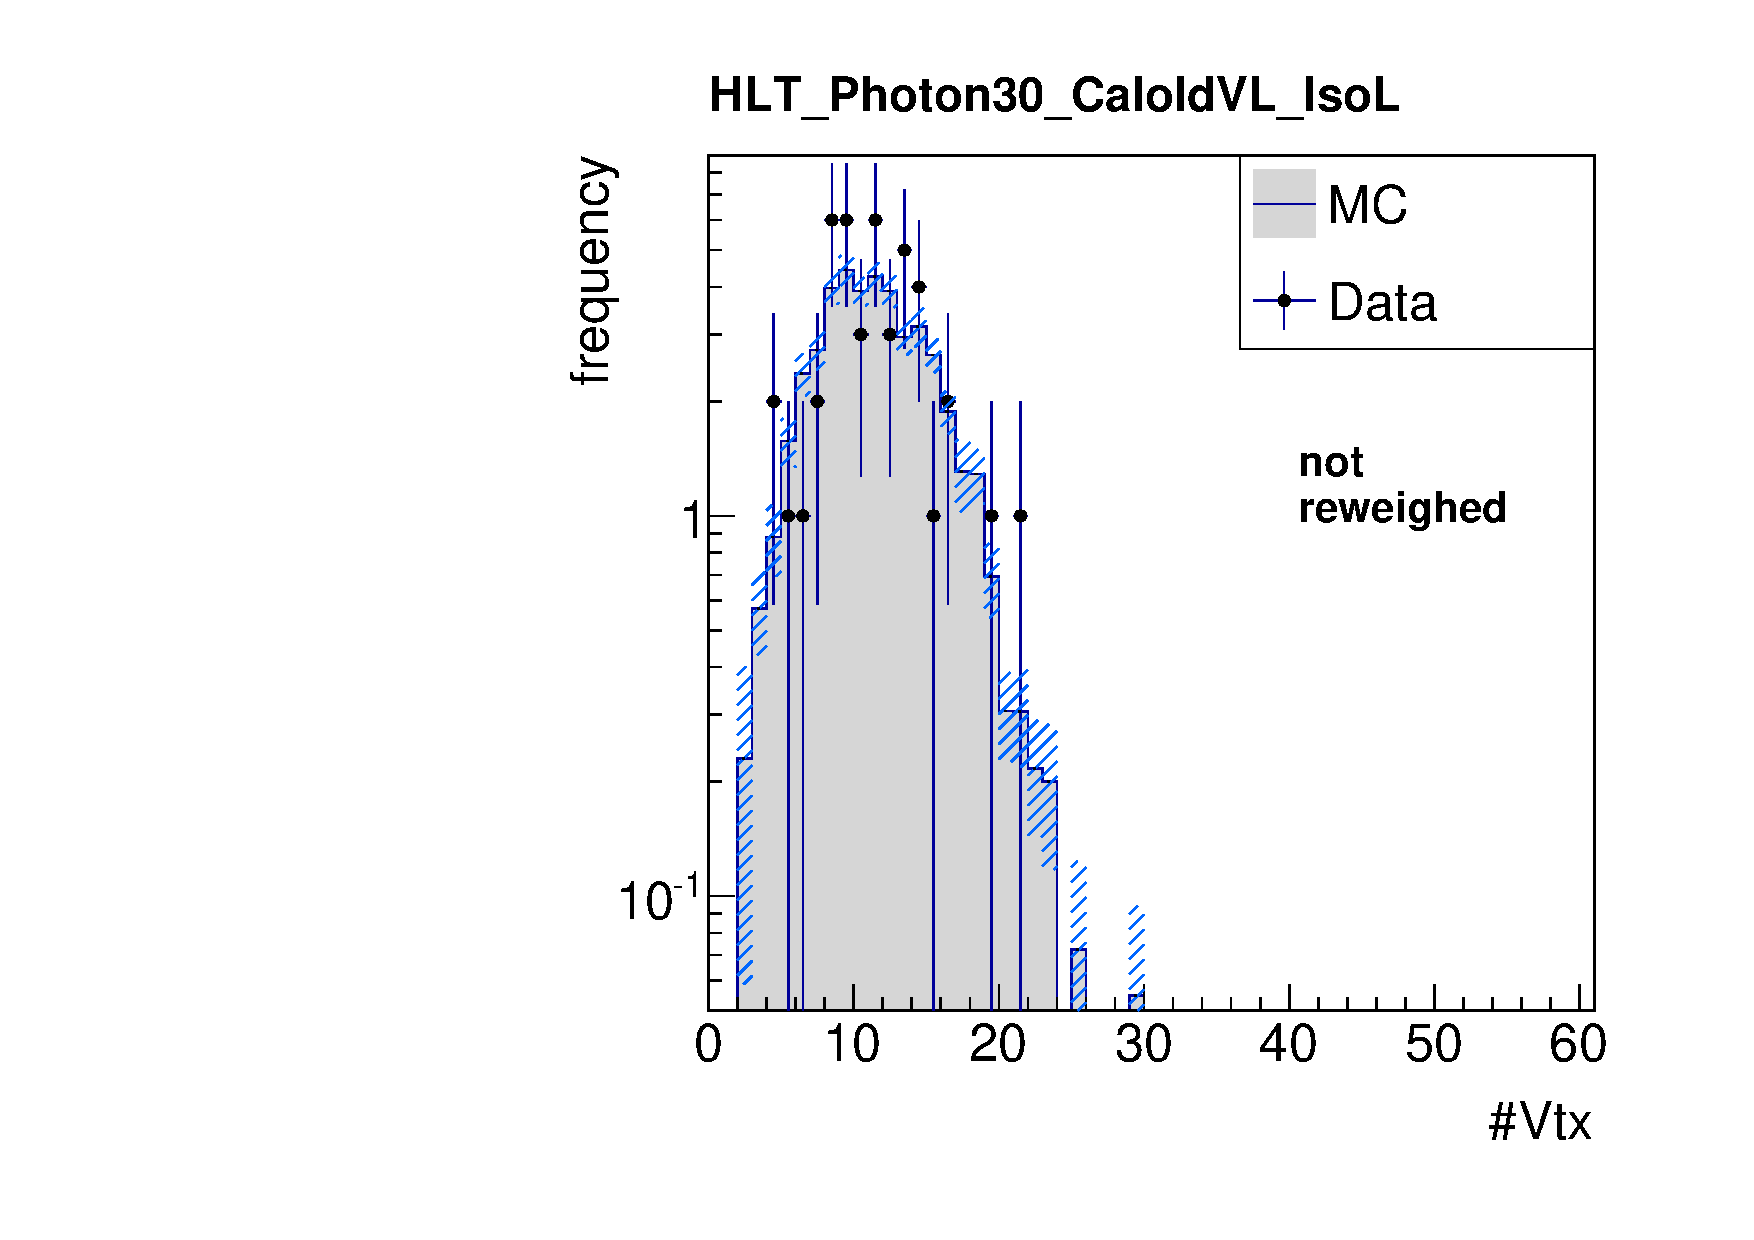
\includegraphics[width=0.22\textwidth]{figures/resolution/eventSelection/NVtxComparisonWoWeights1.pdf}
    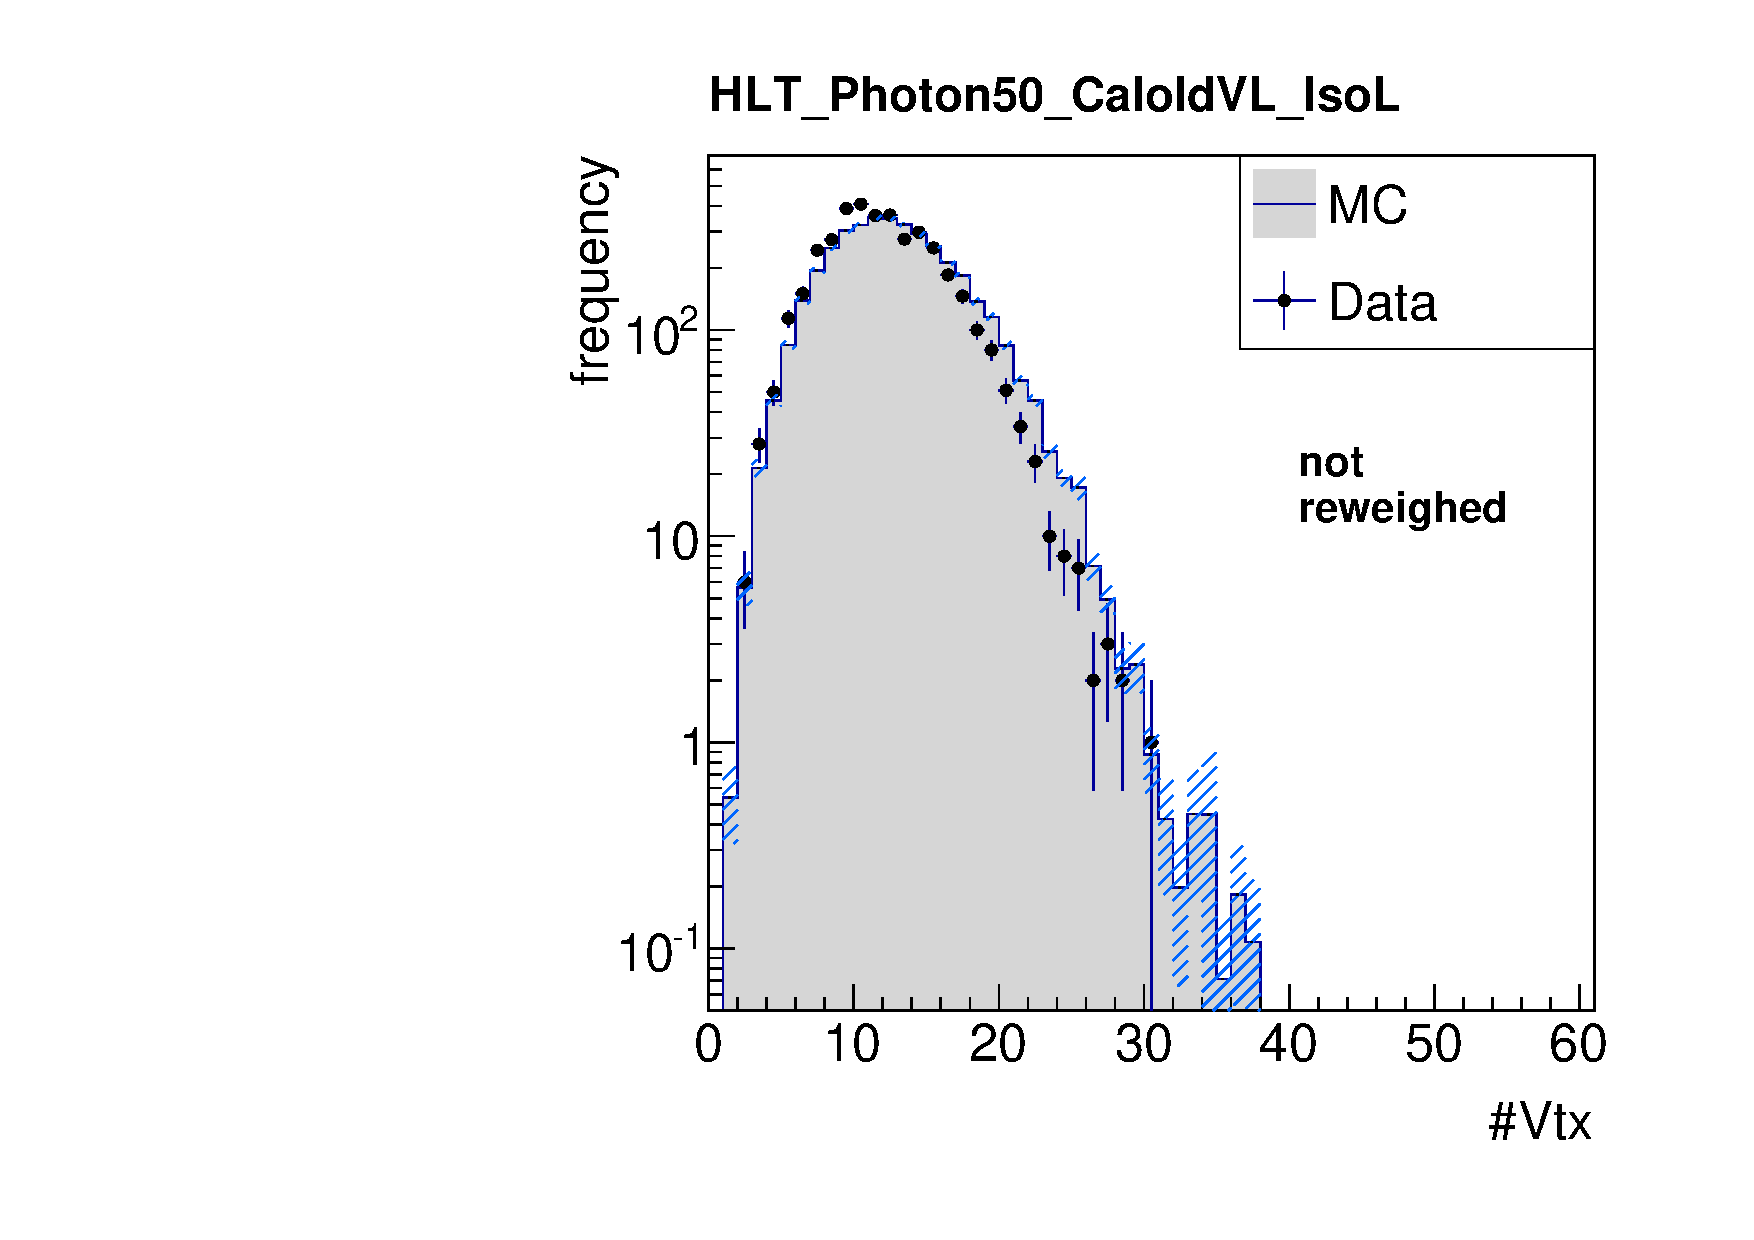
\includegraphics[width=0.22\textwidth]{figures/resolution/eventSelection/NVtxComparisonWoWeights2.pdf}
    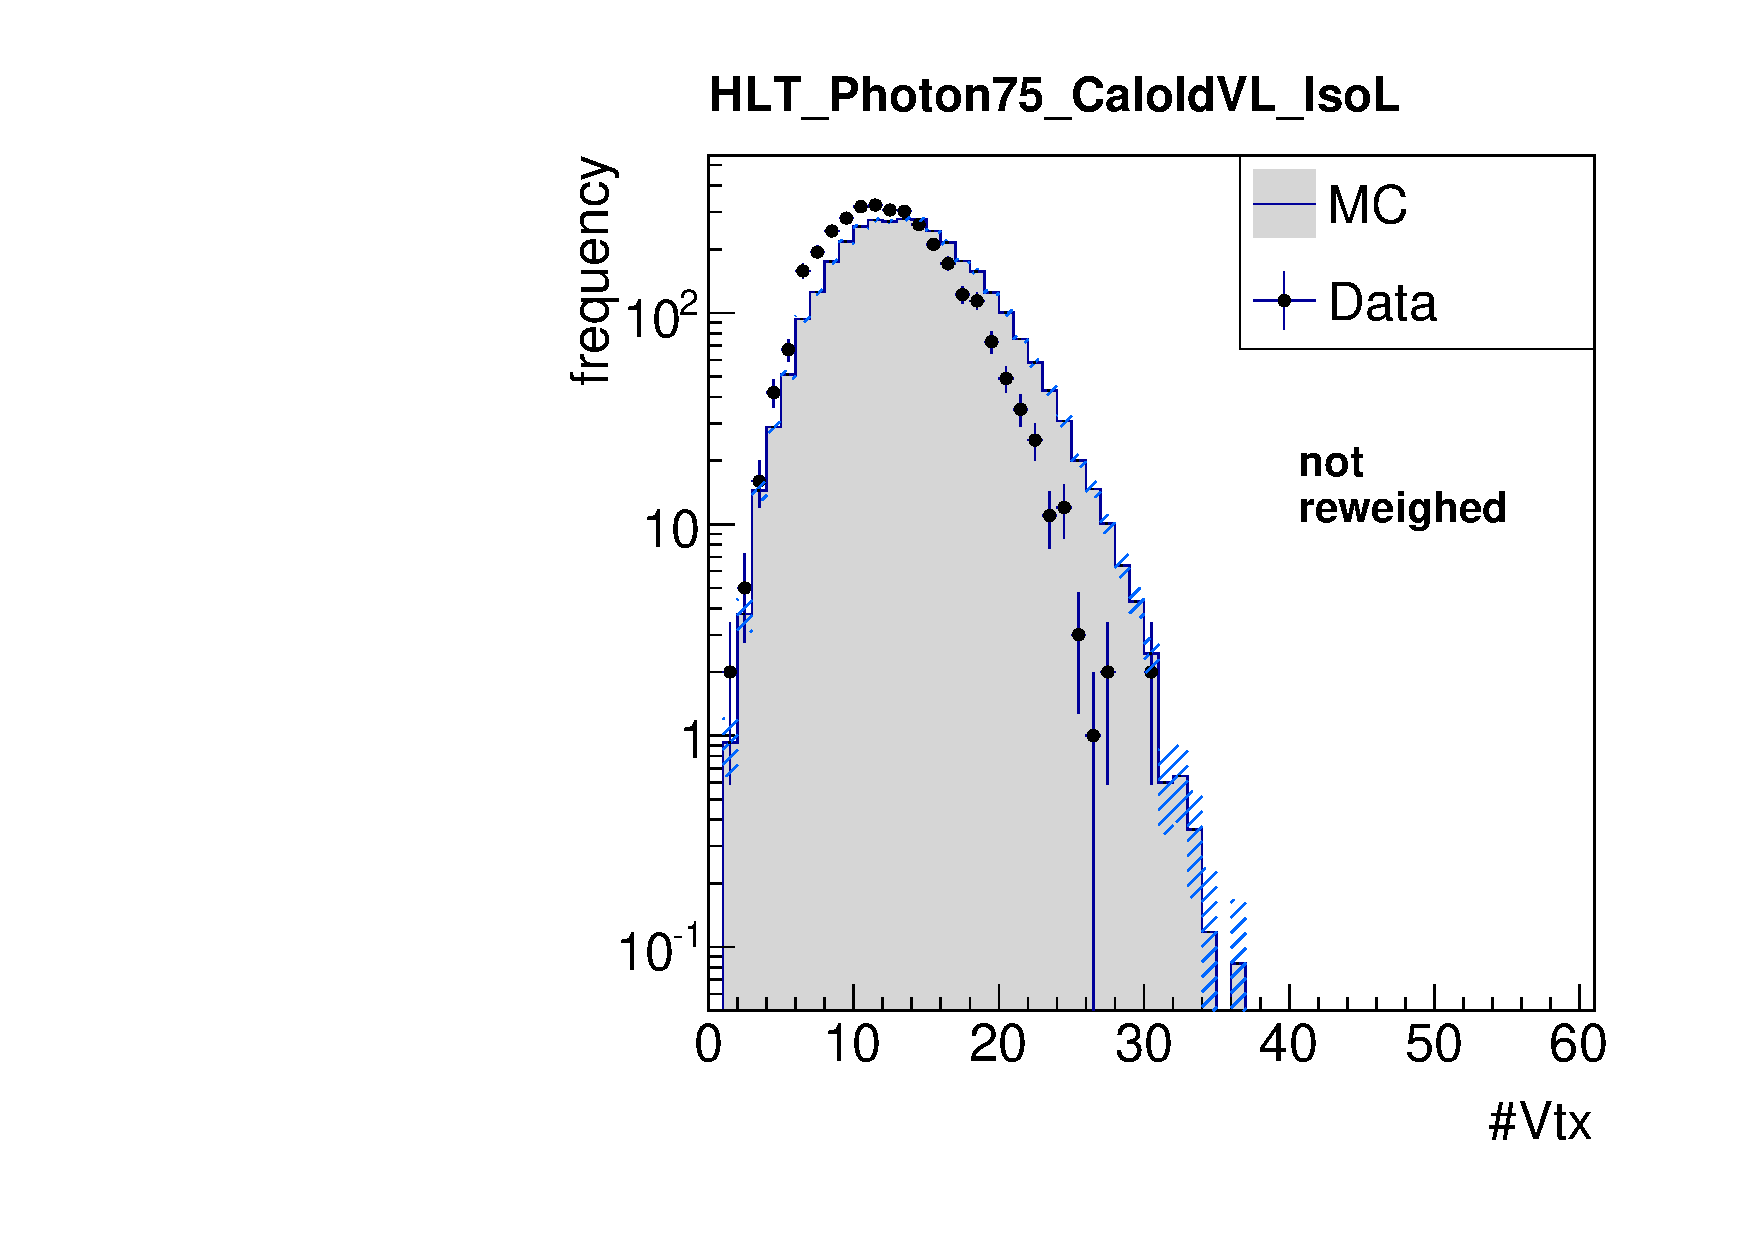
\includegraphics[width=0.22\textwidth]{figures/resolution/eventSelection/NVtxComparisonWoWeights3.pdf}

    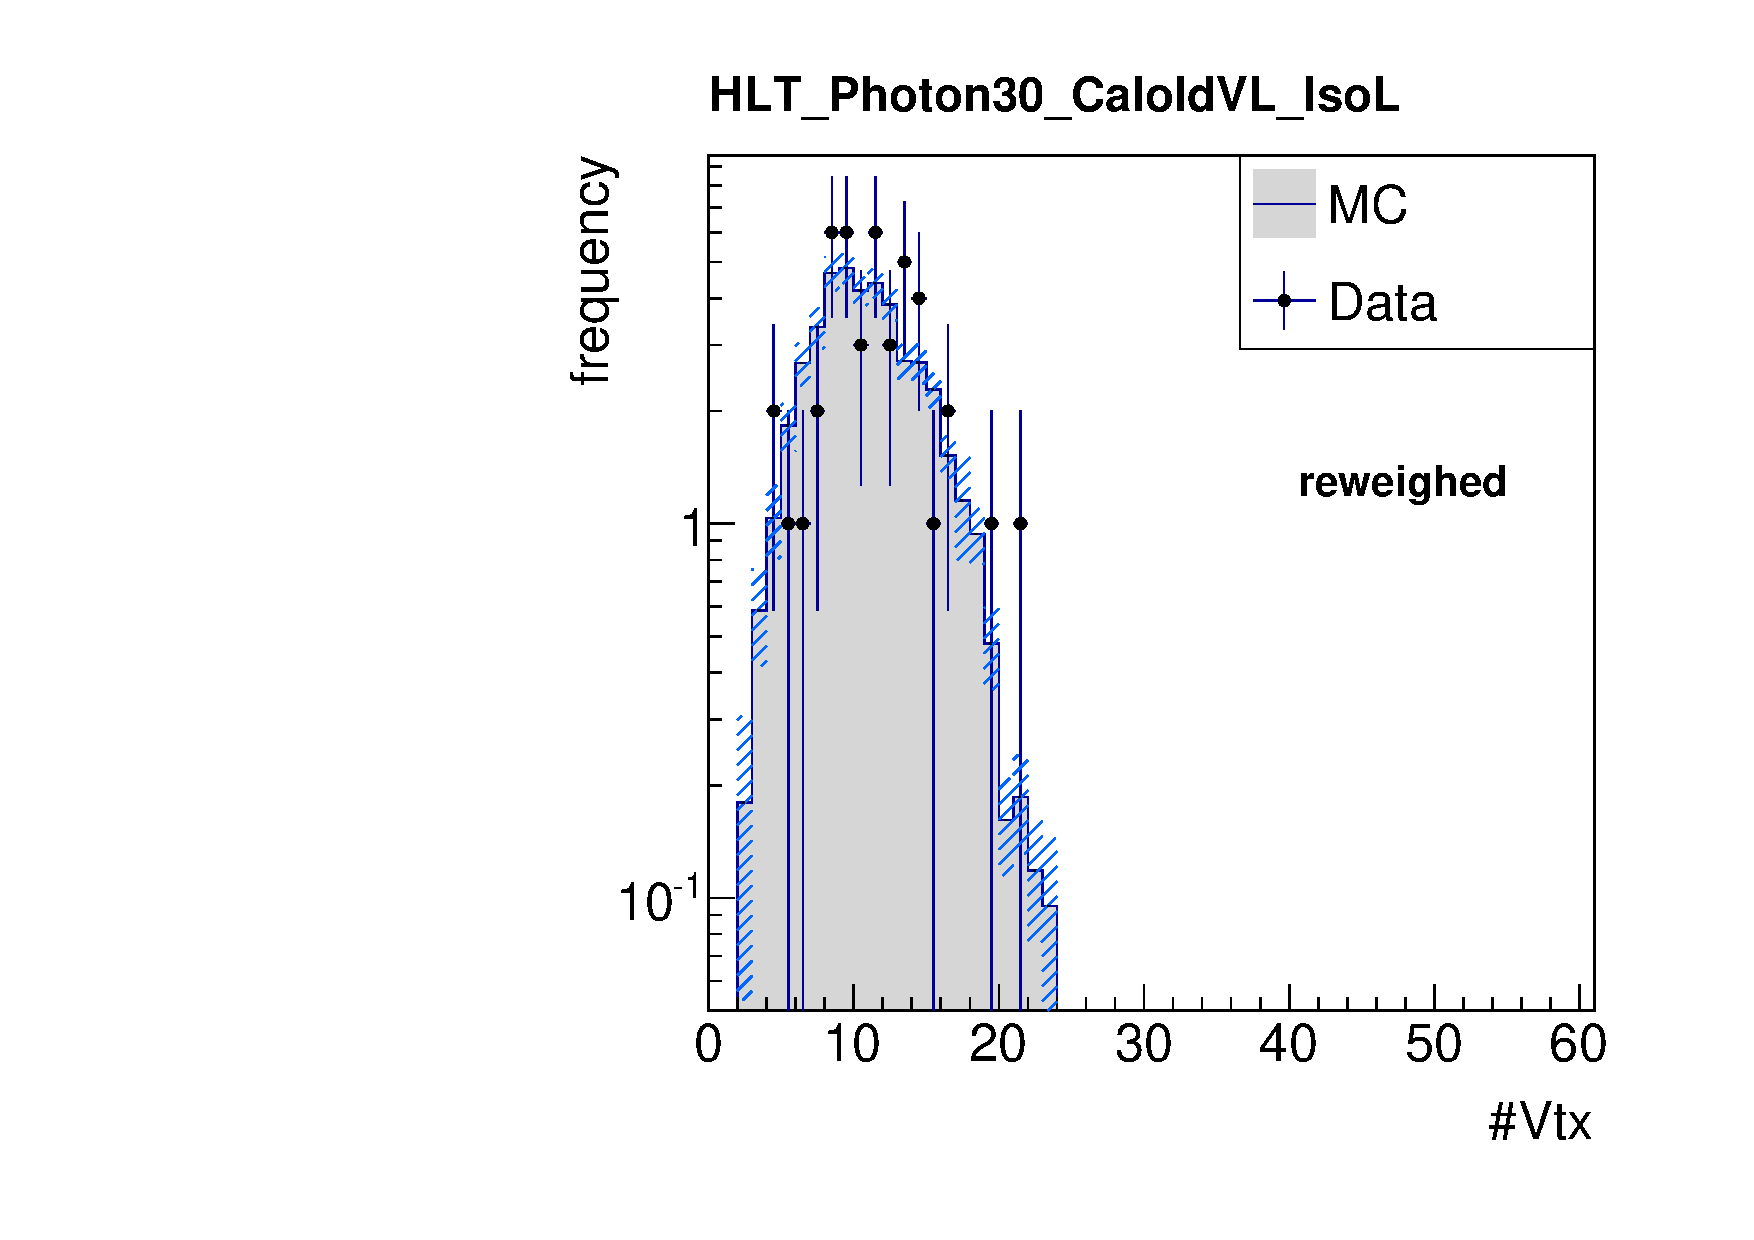
\includegraphics[width=0.22\textwidth]{figures/resolution/eventSelection/NVtxComparison1.pdf}
    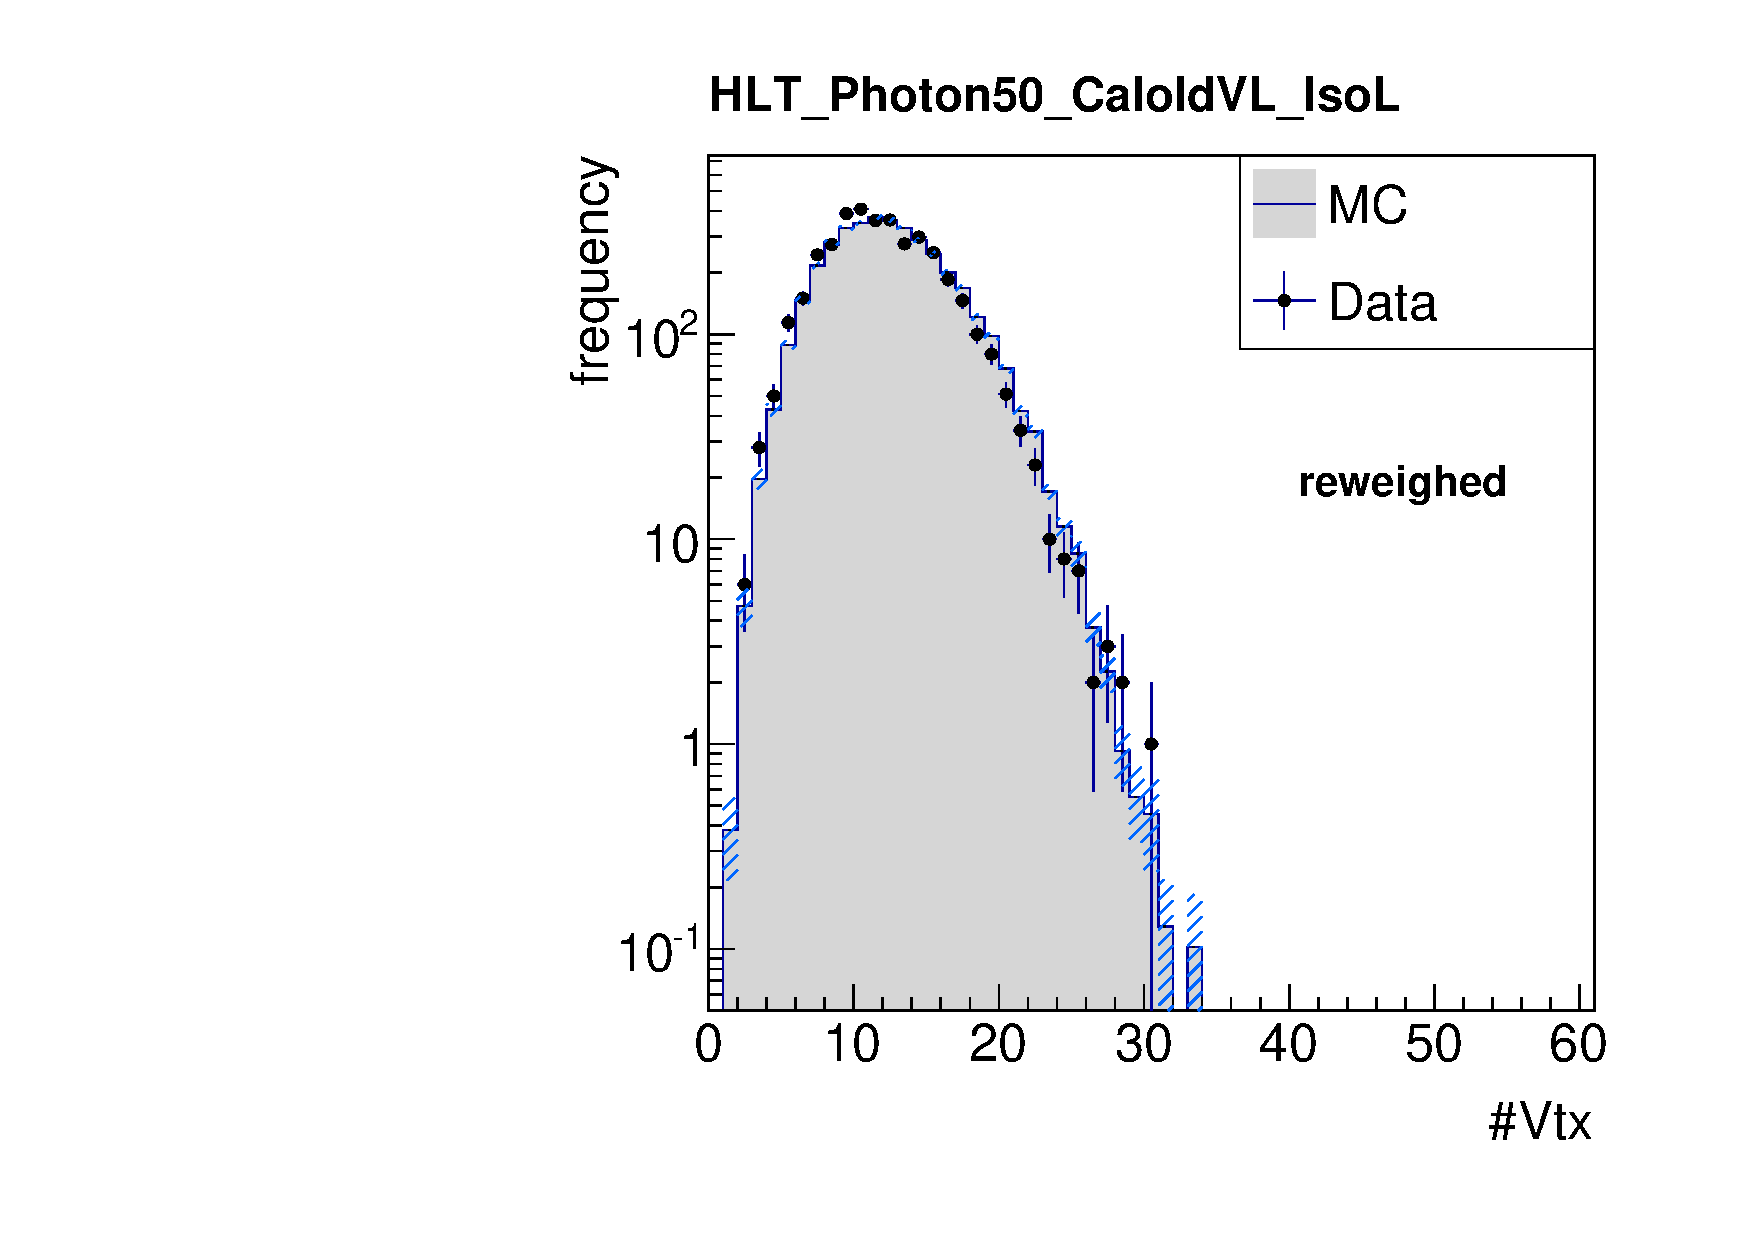
\includegraphics[width=0.22\textwidth]{figures/resolution/eventSelection/NVtxComparison2.pdf}
    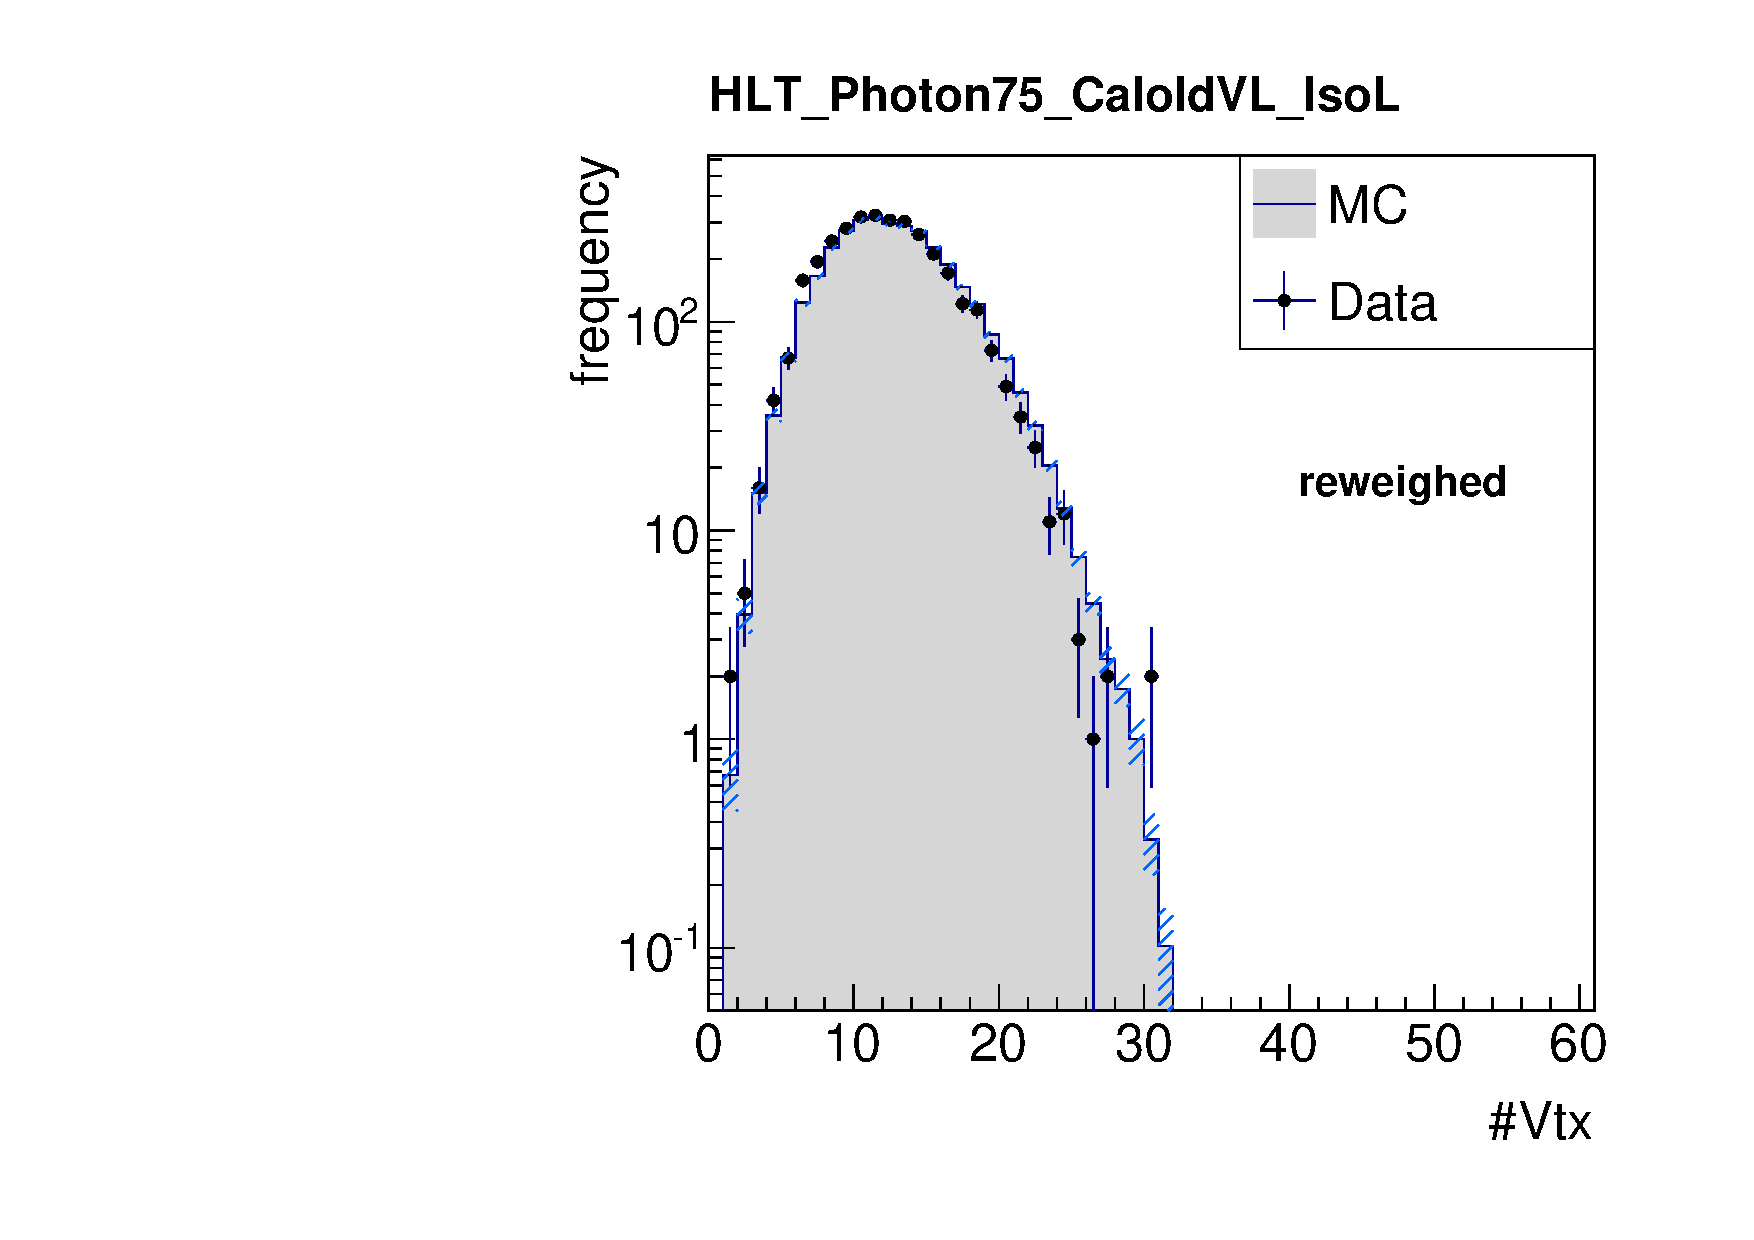
\includegraphics[width=0.22\textwidth]{figures/resolution/eventSelection/NVtxComparison3.pdf}

    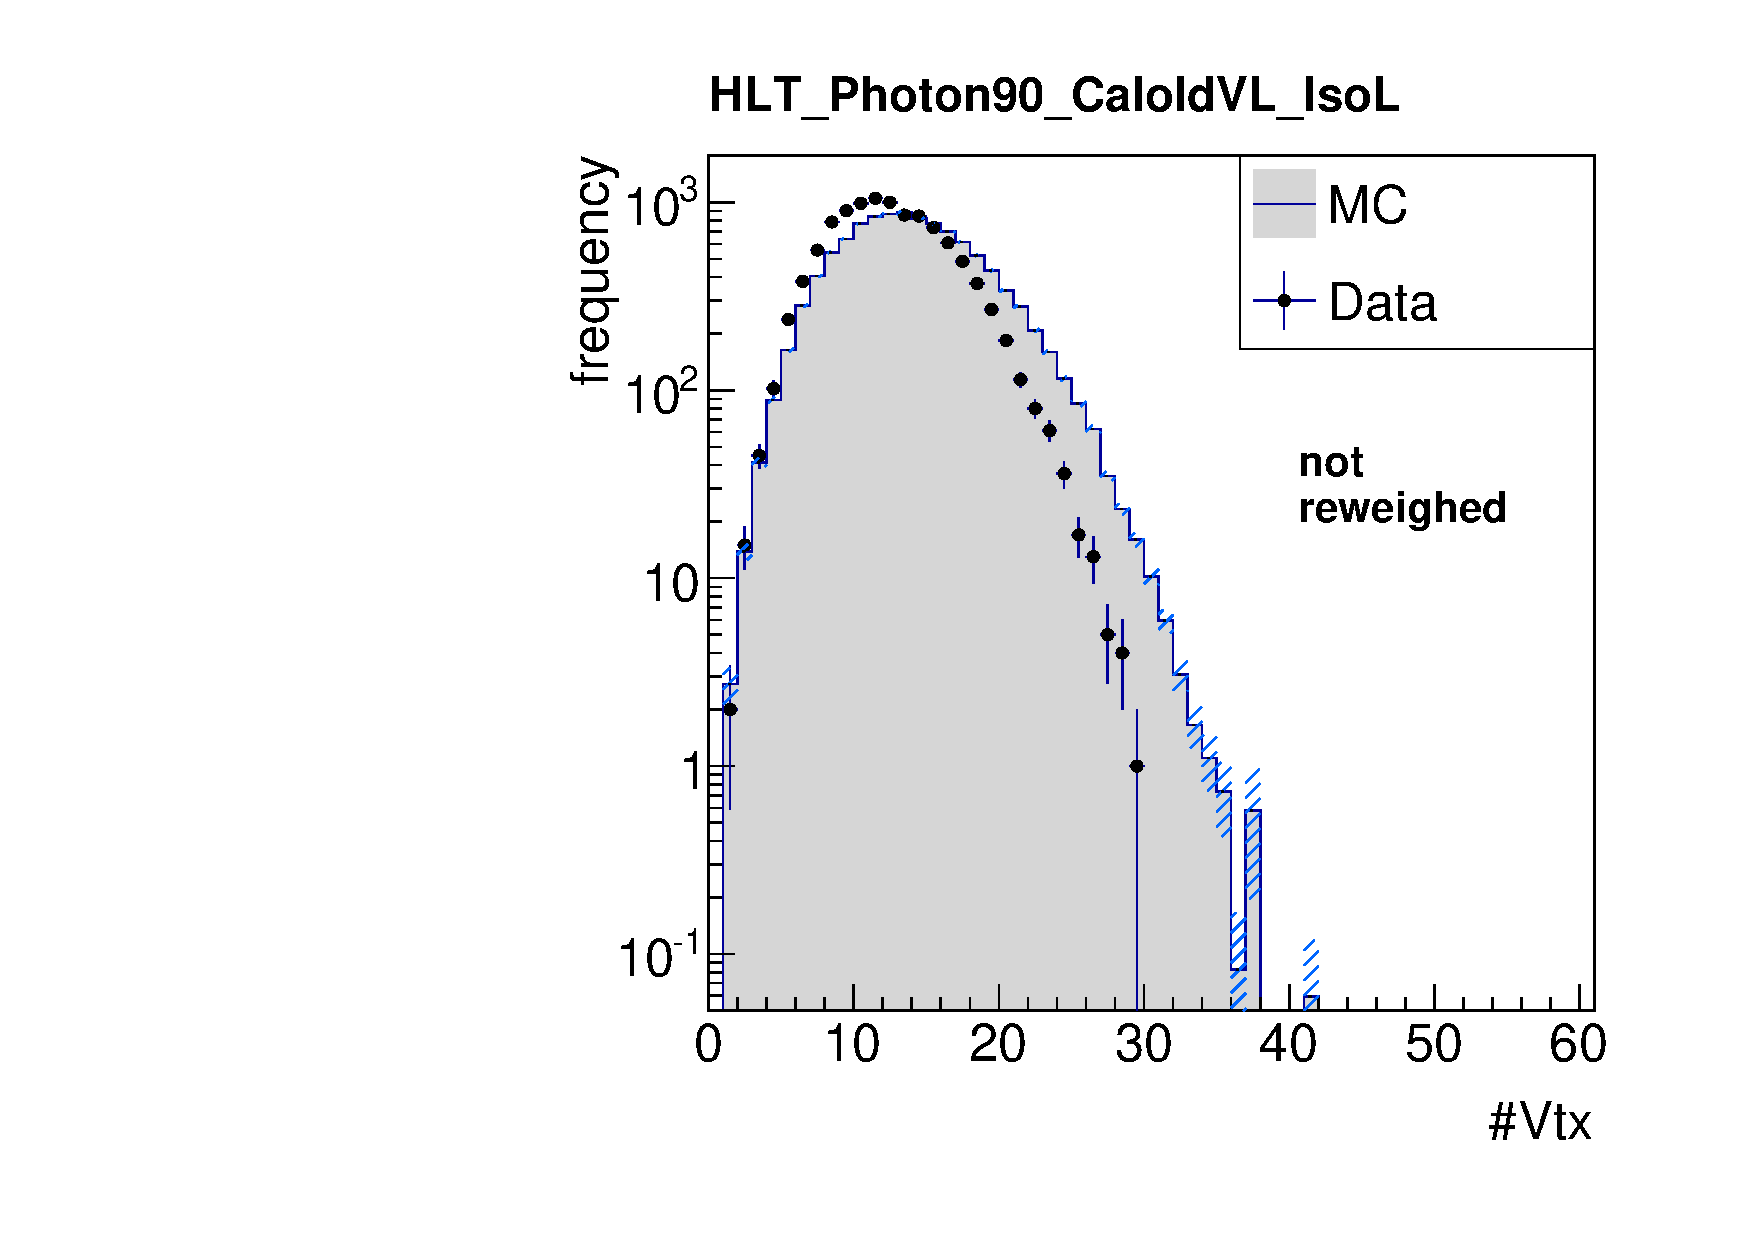
\includegraphics[width=0.22\textwidth]{figures/resolution/eventSelection/NVtxComparisonWoWeights4.pdf}
    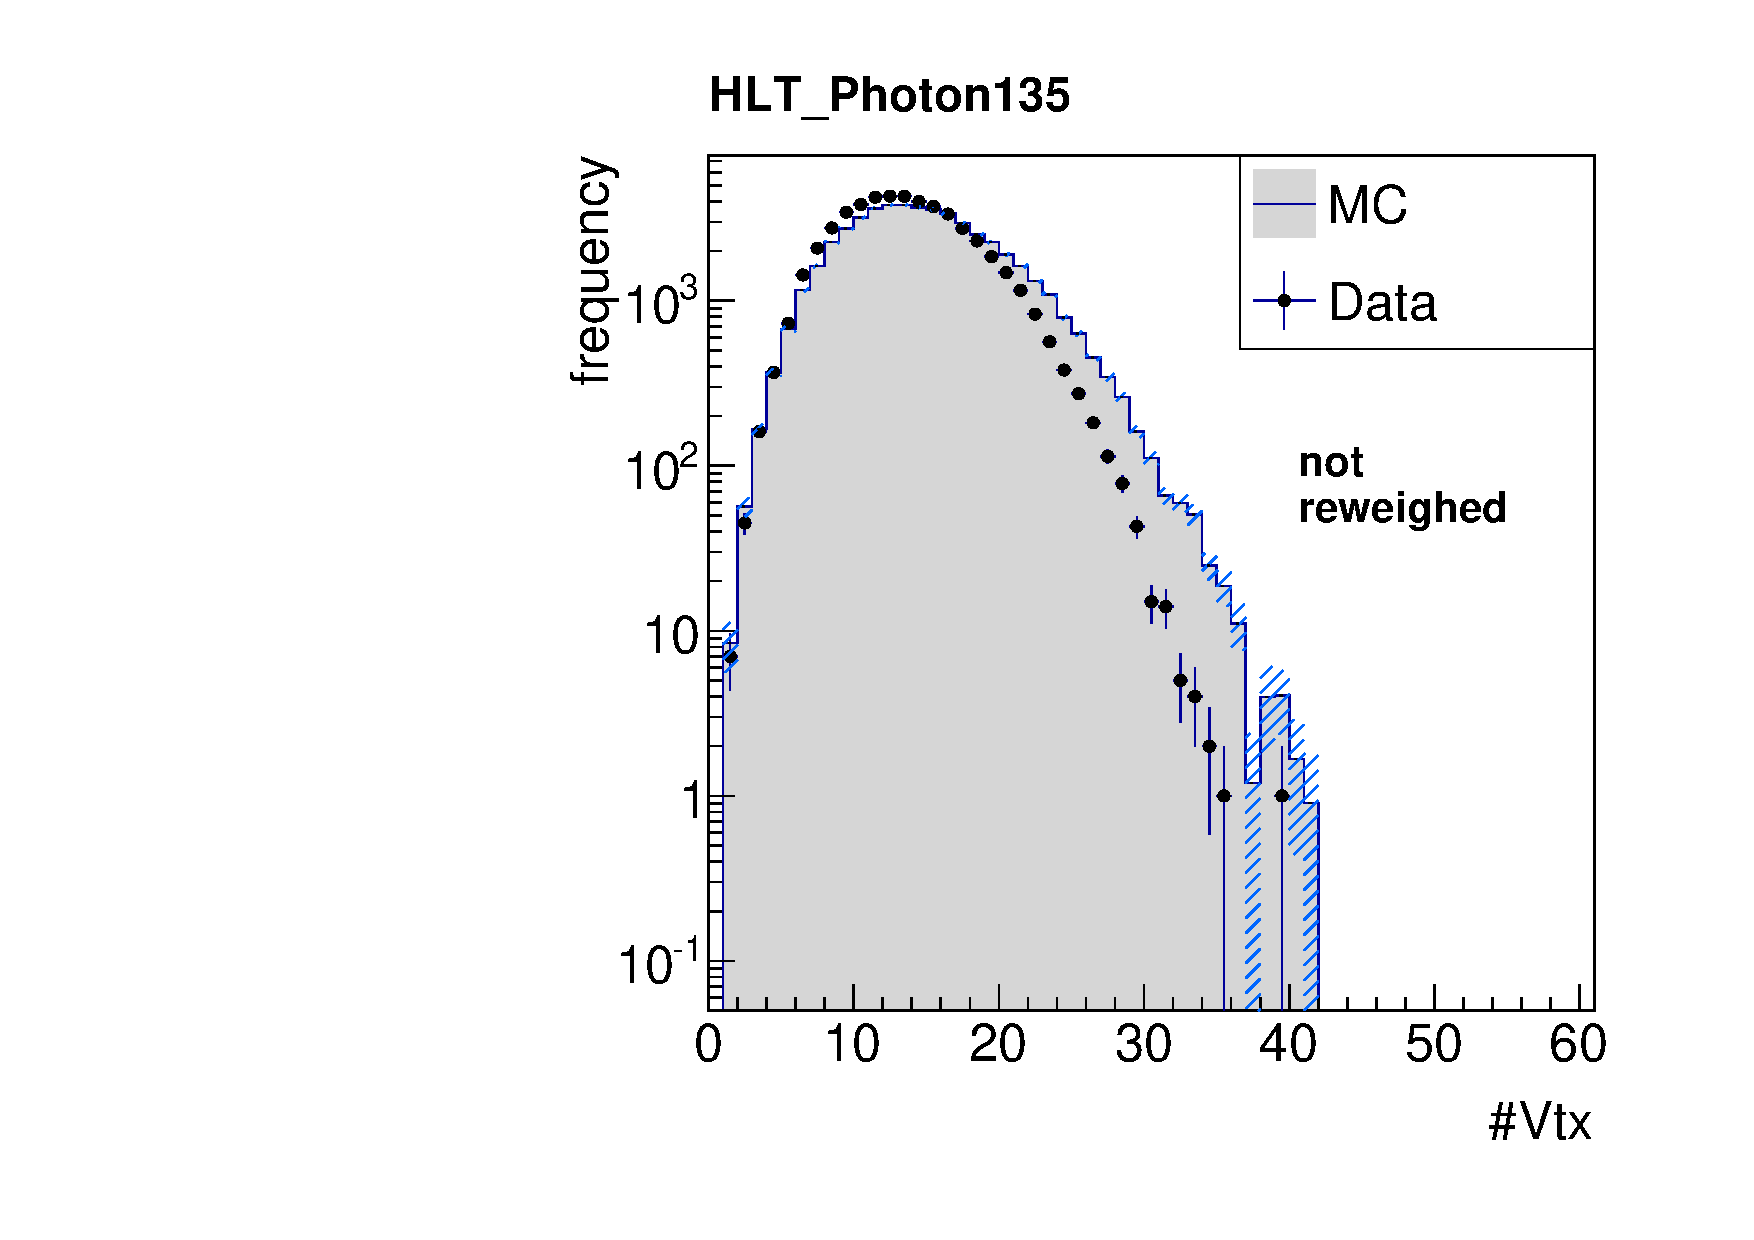
\includegraphics[width=0.22\textwidth]{figures/resolution/eventSelection/NVtxComparisonWoWeights5.pdf}
    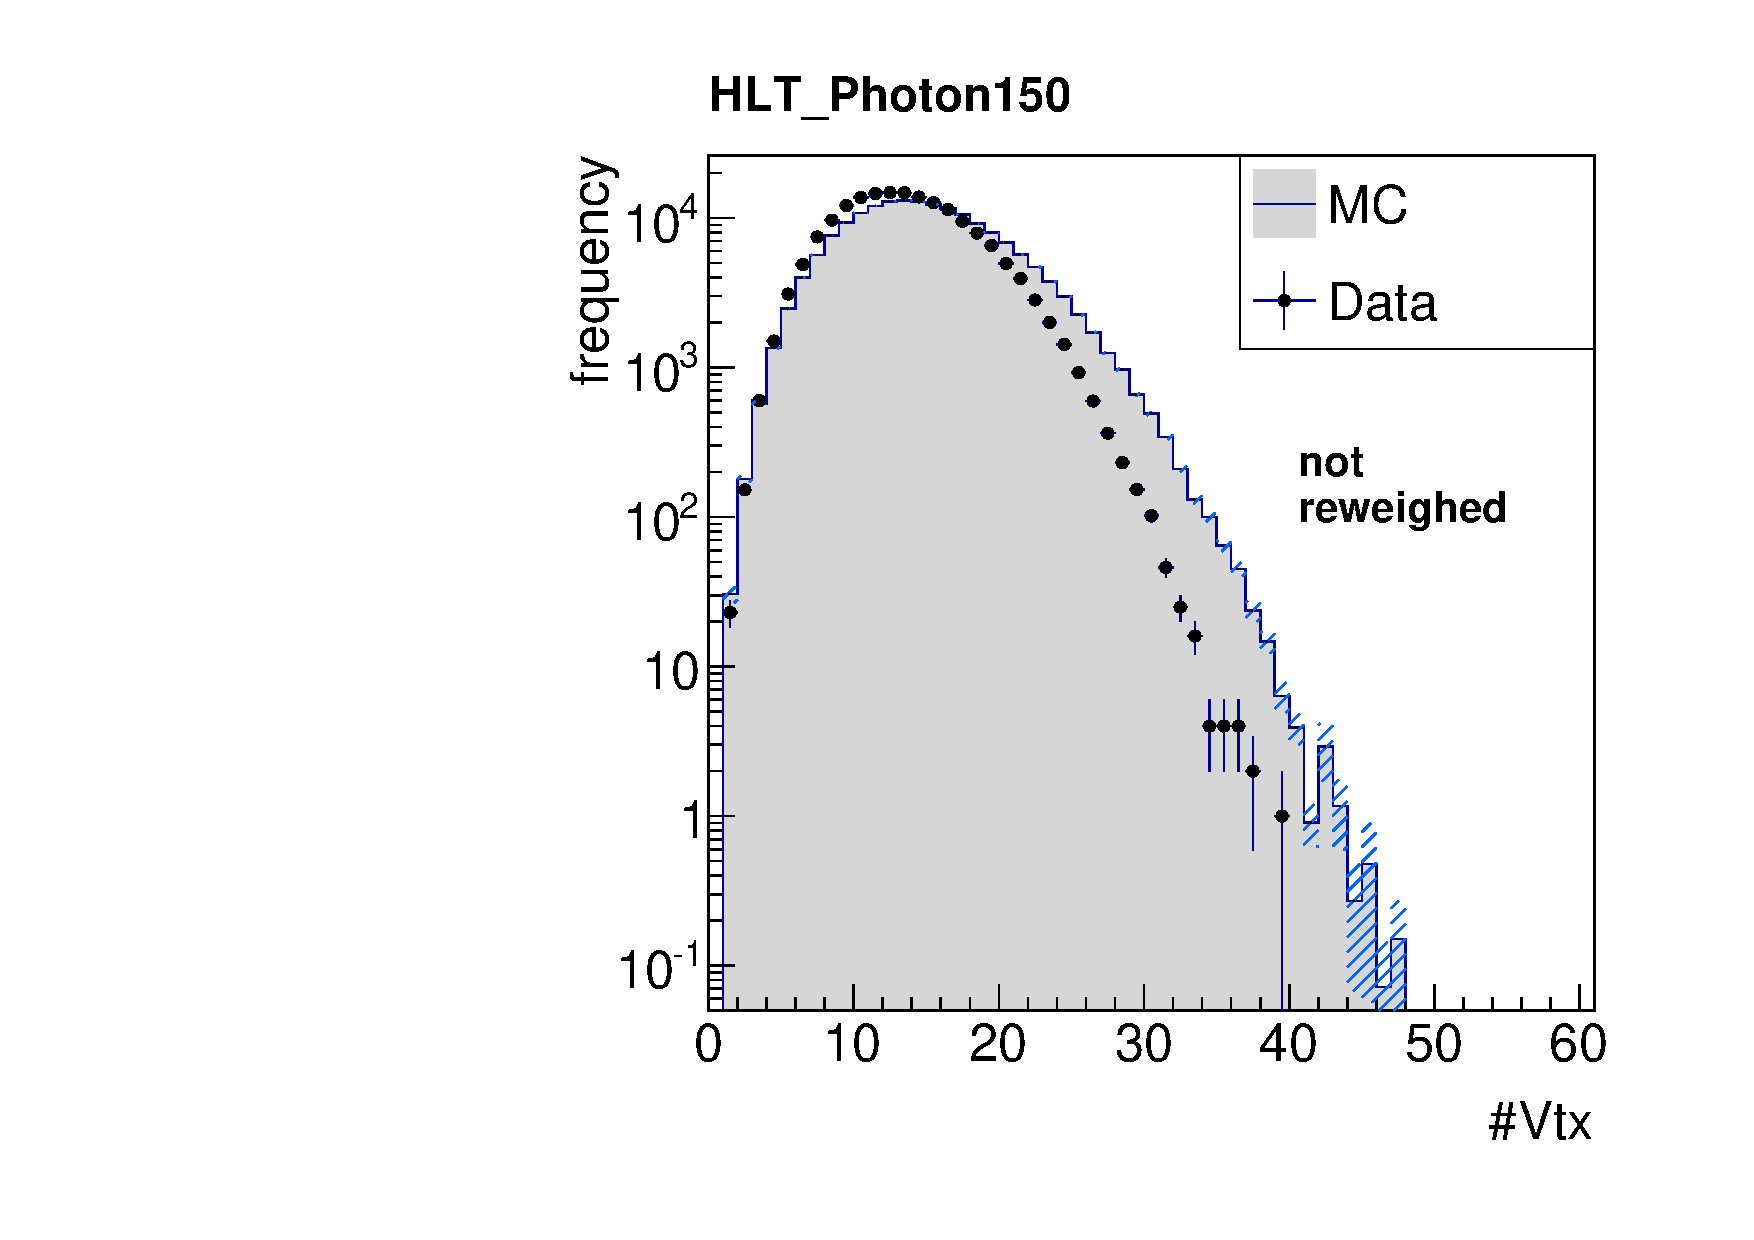
\includegraphics[width=0.22\textwidth]{figures/resolution/eventSelection/NVtxComparisonWoWeights6.pdf}

    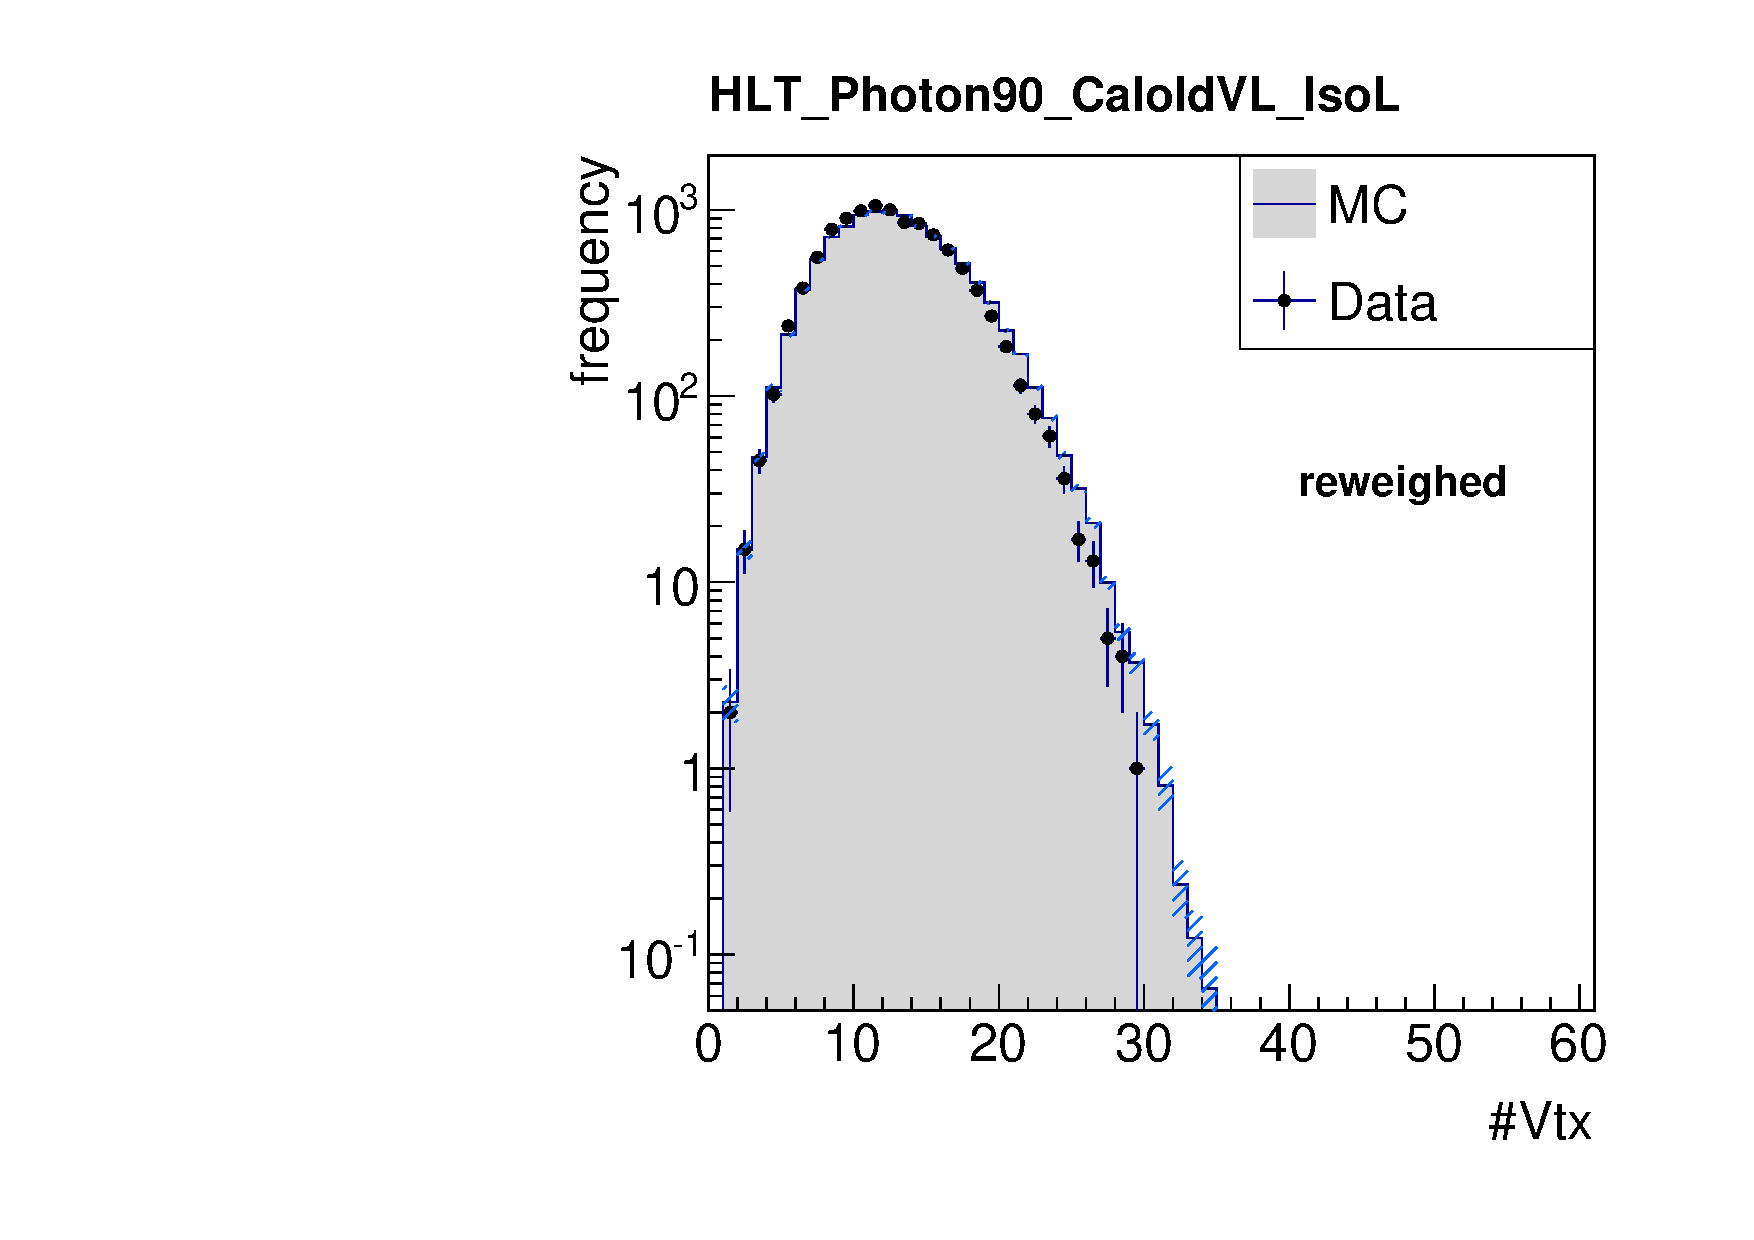
\includegraphics[width=0.22\textwidth]{figures/resolution/eventSelection/NVtxComparison4.pdf}
    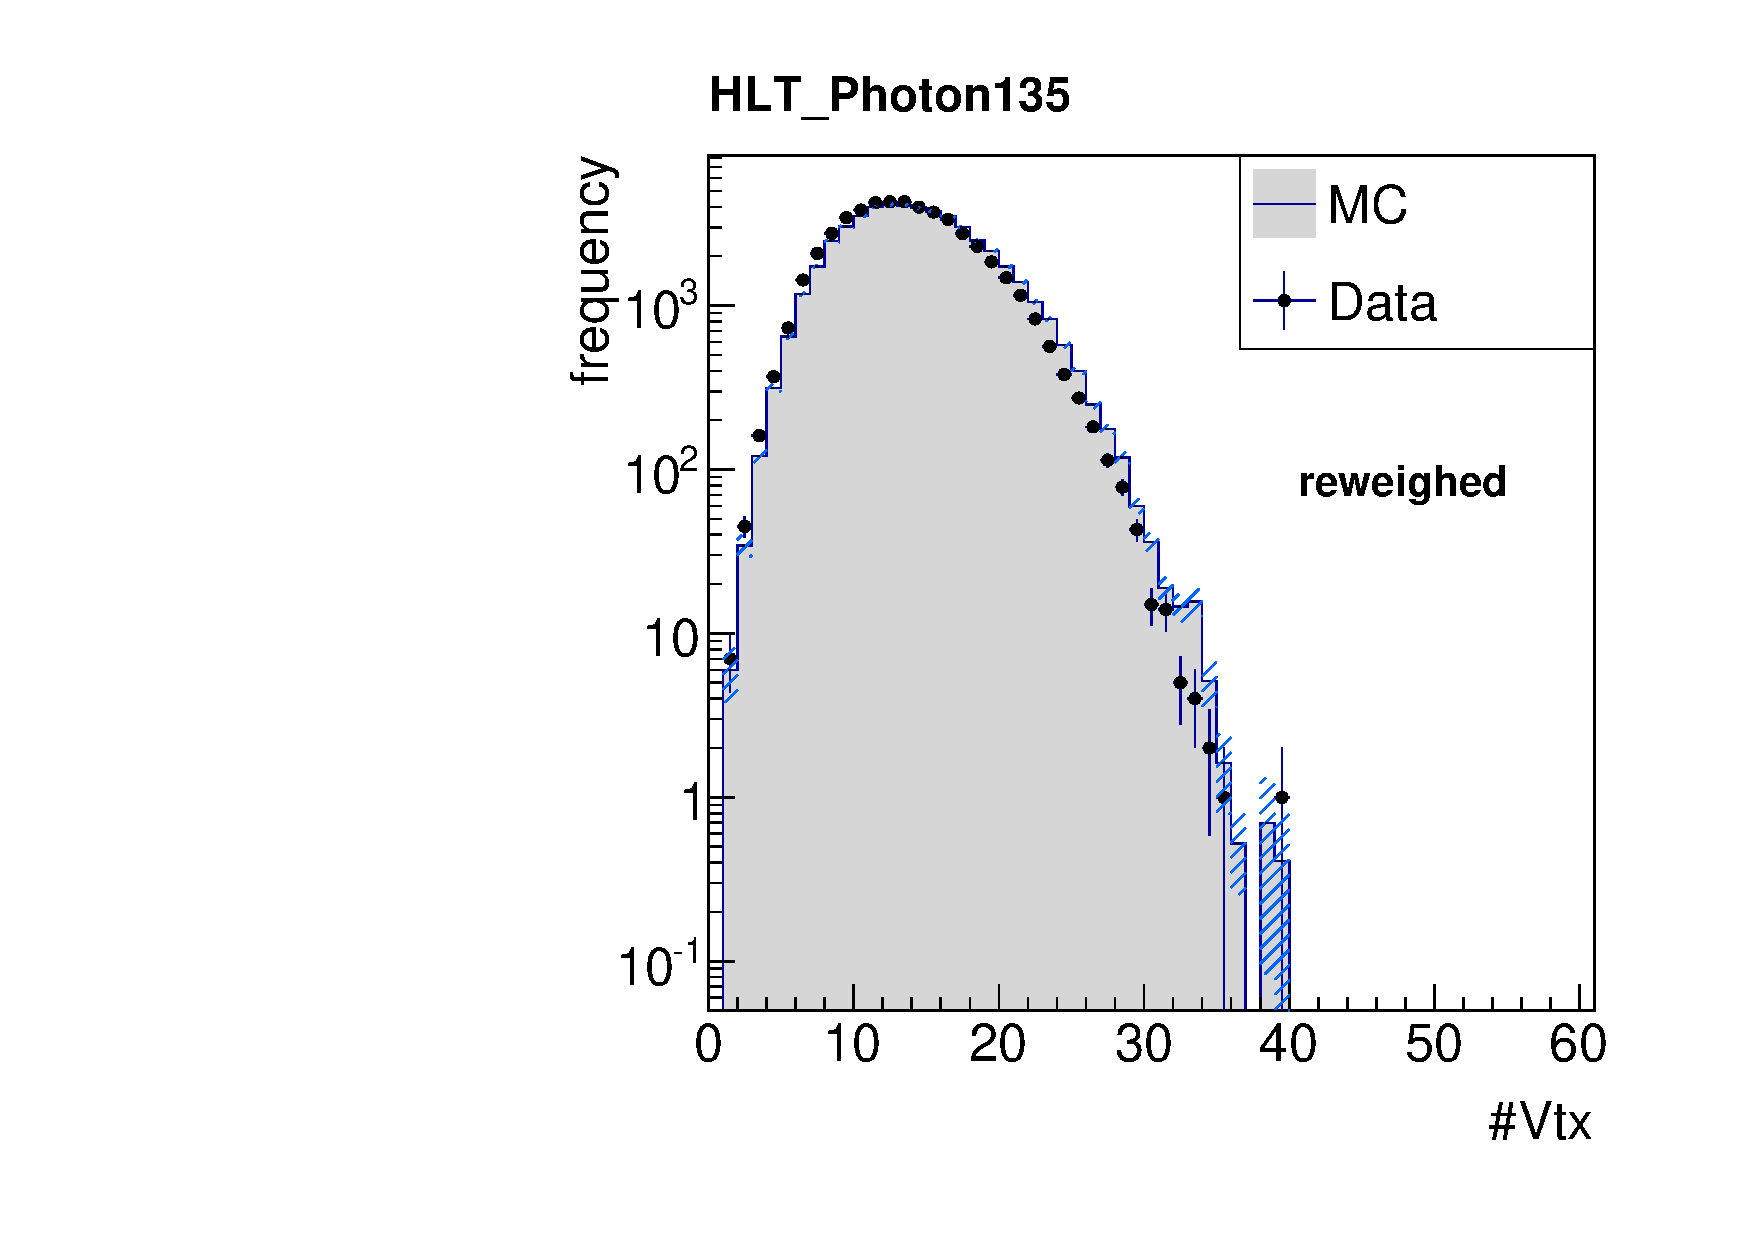
\includegraphics[width=0.22\textwidth]{figures/resolution/eventSelection/NVtxComparison5.pdf}
    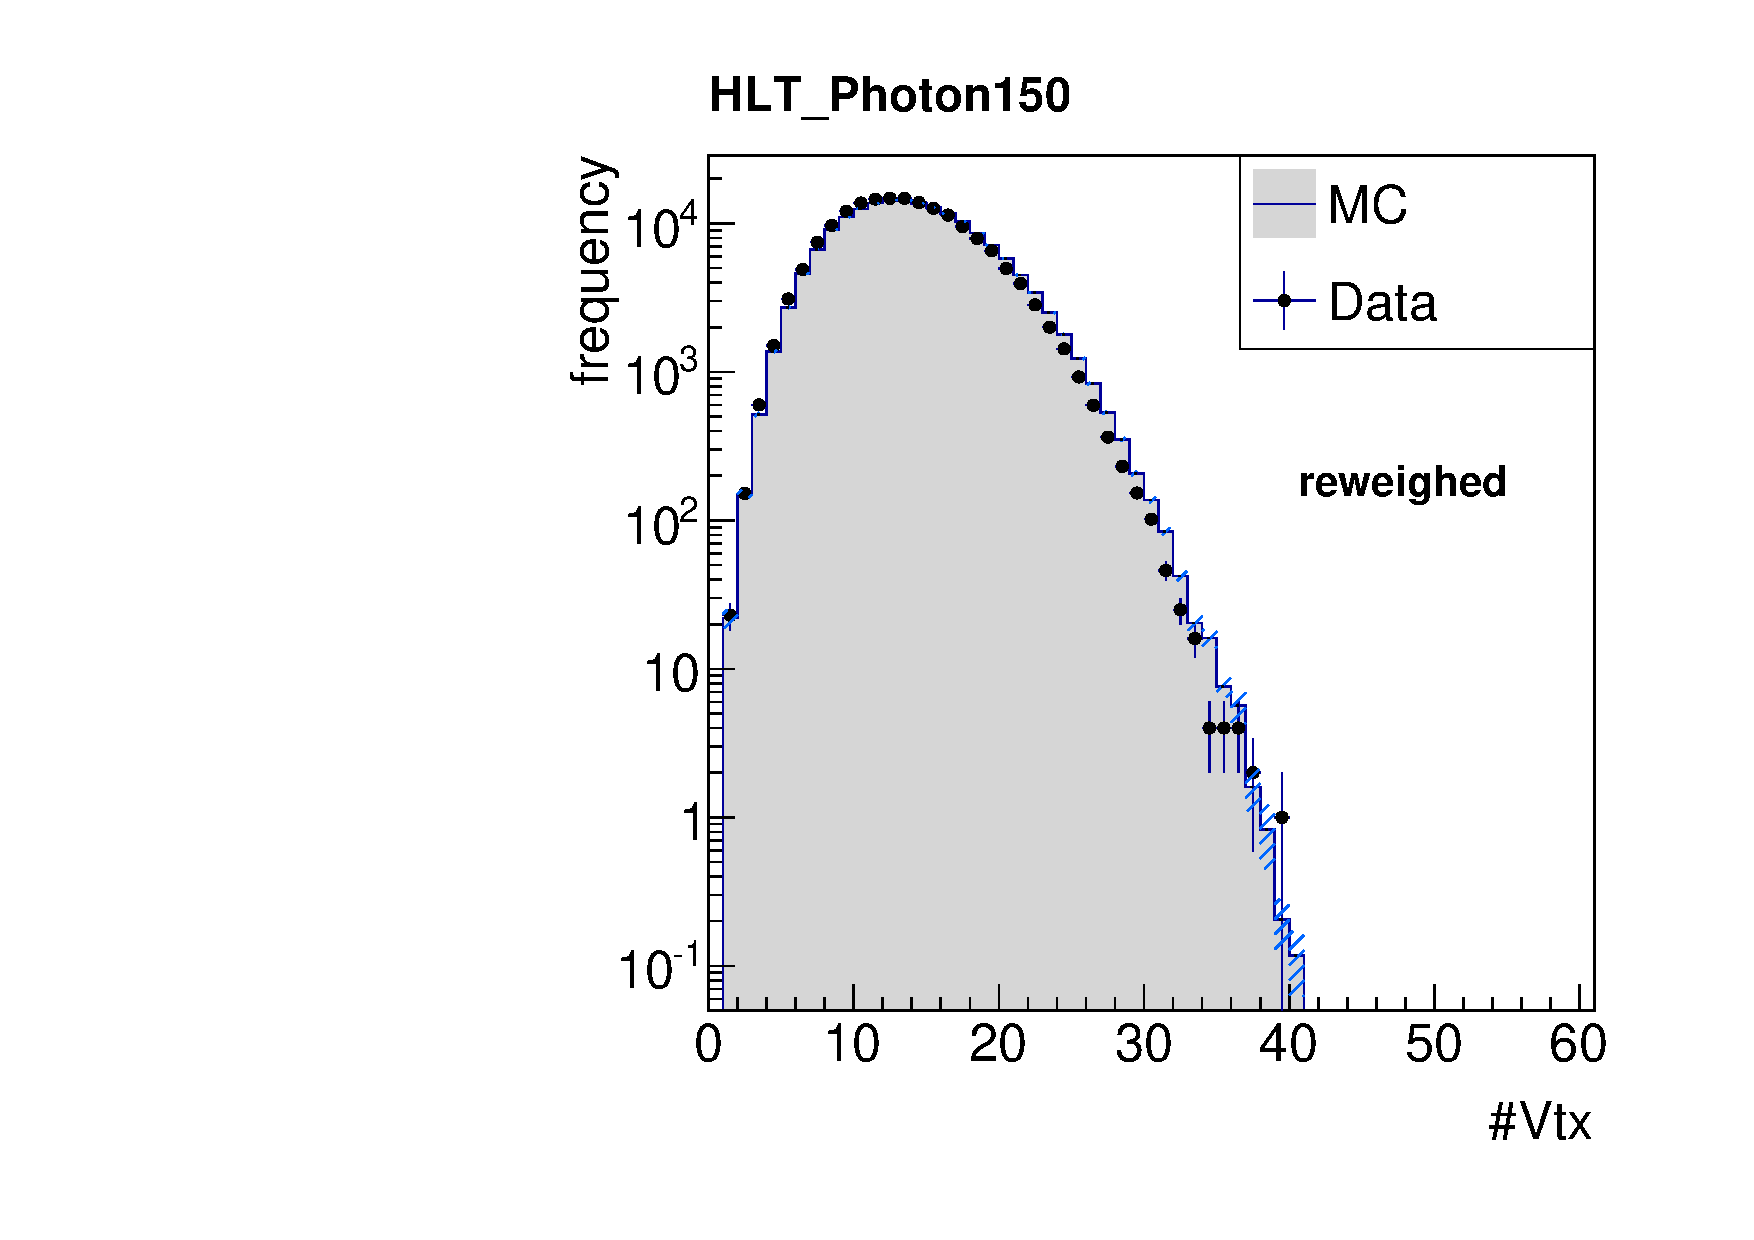
\includegraphics[width=0.22\textwidth]{figures/resolution/eventSelection/NVtxComparison6.pdf}
   \caption{The number of primary vertices in data and simulation before (1st row) and after (2nd row) pileup reweighting for $36\gev < \pt^{\gamma} < 60\gev$ (left), $60\gev < \pt^{\gamma} < 88\gev$ (middle), 
            and $88\gev < \pt^{\gamma} < 105\gev$ (right) and the number of primary vertices in data and simulation before (3rd row) and after (4th row) pileup reweighting for $105\gev < \pt^{\gamma} < 149\gev$ (left), 
            $149\gev < \pt^{\gamma} < 165\gev$ (middle), and $165\gev < \pt^{\gamma}$ (right).}
  \label{res:fig:PUreweighting}
\end{figure}


\section{Summary of all selection requirements}
\label{res:app:eventselection}
FIXME: Update this table and include all details!
\renewcommand{\arraystretch}{1.5}
\begin{table}[htb]
\centering
\caption{Summary of all selection criteria.}
\label{res:tab:selection}
\makebox[0.99\textwidth]{
\begin{tabular}{l | c | l}
\multicolumn{3}{c}{} \\
\toprule
  &      Selection                                               & Further specifications                                                                 \\
\midrule
1.&  Leading Photon  & See table \ref{res:tab:PhotonIsolation} in section \ref{res:sec:EventSelection} for the specific selection requirements            \\
2.&  Leading Jet is tight                                        & See in section \ref{res:sec:EventSelection} the specific selection requirements    \\
3.&  $\pt^{\text{1st jet}} > 10\gev$                             &                                                                                       \\
4.&  $\pt^{\text{2nd jet}} > 10\gev$                             &                                                                                       \\
5.&  $\eta^{\gamma}<1.3$                                         &                                                                                       \\
6.&  $\Delta \Phi \left(\text{1st jet}, \gamma \right) > 2.95 $  &                                                                                       \\
7.&  $\frac{\pt^{\text{2nd jet}}}{\pt^{\gamma}} < 0.20$          & With the following binning: [0,0.075,0.1,0.125,0.15,0.175,0.2]                        \\
8.&  Trigger $\pt^{\gamma}$ bounds                               & With the following bounds: [22,36,60,88,105,148.5,165,176,$\inf$]                     \\
\bottomrule
\multicolumn{3}{c}{} \\
\end{tabular}}
\end{table}

